\documentclass[../../main.tex]{subfiles}

% 

\begin{document}
\chapter{Koincidenčné systémy}

\section{Stručný úvod}
Súčasné fyzikálne deje je možné študovať v tzv. koincidenčných meraniach. Základom je elektronický, tzv. koincidenčný blok, na ktorého výstupe sa objaví impulz iba vtedy, keď sú na jeho vstupy privedené impulzy, ktoré sa časovo prekrývajú. Súčastnosť namerania dejov je vždy zaťažená istou chybou, ktorá je daná časovou fluktuáciou vytvárania signálu v detektoroch a vlastnou časovou rozlišovacou chybou koincidenčných zariadení. Celkové časové rozlíšenie súčasných dvoch a viacerých dejov je dané hlavne rýchlosťou vytvárania signálu v detektoroch a pohybuje sa pri dnešnej technike v rozmedzí $10^{-6} - 10^{-10}\,s$. Koincidenčný obvod je elektronický obvod, ktorý slúži k detekcii pravých koincidencii a k odlíšeniu rozptýlených či náhodných koincidencii. V závislosti od účelu experimentu môžu byť tieto udalosti odmietnuté (anti-koincidencia) alebo prijaté (koincidencií).

Hlavnou myšlienkou koincidenčnej detekcie pri spracovaní signálu je nasledujúca skutočnosť: ak detektor zaznamená pulz, je potom istá pravdepodobnosť ($p$), že sa jedná o šum. Ak ale pulz zaznamenajú zároveň dva detektory potom pravdepodobnosť, že sa jedná o šum bude $p^2$. Za predpokladu, že $p \leq 1$ dostávame, že výsledná pravdepodobnosť zaznamenania šumu bude kvôli koincidenčnému meraniu menšia (napríklad ak $p=0.1$, potom $p^2=0.01$).

Jedným z rozhodujúcich faktorov je výška pulzov, ktorých filtrácia prebieha v pulzne výškových analyzátoroch. Tieto analyzátory prepustia iba pulzy, ktoré pochádzajú z častíc, ktoré mali dostatočne veľkú energiu. Ďalším rozhodujúcim faktorom pre koincidenčný obvod je signál z časového diskriminátora, ktorý zaznamenáva časy dopadu jednotlivých častíc. Koincidenčný obvod potom vyhodnotí signály s adekvátnou amplitúdou prichádzajúcich z protiľahlých detektorov a rozhodne, či časový rozdiel medzi registráciou oboch dopadov spadá do koincidenčného časového okienka. 

V tom najideálnejšom prípade by sme dva signály z detektorov mali zaznamenať v rovnakom čase. Avšak v reálnom svete tomu tak nieje pretože fyzikálne udalosti sú vždy spojené s časom, čo je vo svojej podstate spojitý parameter. Meranie spojitého parametra, akým je čas, vyžaduje určitú analógovo-digitálnu konverziu, čo spôsobuje určité chyby v kvantifikácii. Technicky sa koincidencia označuje ako výskyt dvoch udalostí A a B, ku ktorým dochádza v definovanom časovom rozpätí. Toto rozpätie sa nazýva koncidenčné okienko $T_c$. Koincidencia preto nastáva vtedy, keď pre časy výskytu udalostí A a B, $t_A$ a $t_B$, platí nasledovné:
$$ -T_c < t_A-t_B < T_c.$$

Vo všeobecnosti, mnoho koncidenčných detekčných systémov používaných v medicíne, kvantovej fyzike alebo optike pozostáva z dvoch hlavných časti: 
\begin{itemize}
\item jednotlivých detektorov, ktoré zaznamenávajú jednotlivé eventy 
\item koncidenčného detektora
\end{itemize}
Všeobecná schéma takéhoto systému je znázornená na obrázku (\ref{em8:fig:koncidencia}). 

Pozitrónová emisná tomografia (PET) napríklad používá detektory scintilačného žiarenia, zatiaľ čo niektoré oblasti výskumu kvantovej mechaniky využívajú moduly na počítanie jednotlivých fotónov tzv. Single Photon Counting Modules  (SPCM), ktoré detekujú emitované fotóny. Výstupné porty detektorov zabezpečujú signálny impulz po úspešnej detekcii udalosti, t.j. príchodu fotónov alebo lúčov.

Druhou hlavnou časťou detekcie koincidencie je následná fáza spracovania, ktorá sleduje výstupné impulzy vyššie uvedených detektorov. Ak impulzy dvoch (alebo viacerých) detektorov dorazia vo zvolenom časovom okienku, systém ich považuje za koincidencie.
Táto fáza prebieha v tzv. field-programmable gate arrays (FPGAs).

\begin{figure}[!h]
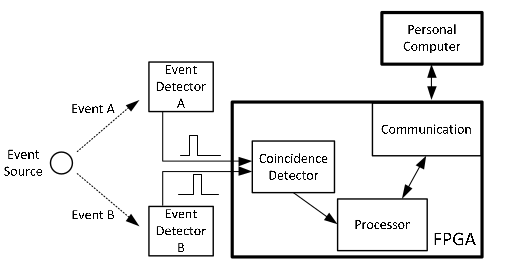
\includegraphics[width=0.9\textwidth]{emsf-08-koincidencia.png}
\centering
\caption{Všeobecná schéma pre koincidenčnú detekciu.}
\label{em8:fig:koncidencia}
\end{figure}

Základná metóda určovania koincidencie je nasledovná: prichádzajúce eventy (t.j. pulzy vysielané detektormi) sa jednoducho privádzajú do tzv. AND brány. Ak sú tieto pulzy zaznamenané v rozsahu koincidenčného okienka tak sa potom aktivuje výstupný port AND brány. Tento prístup však čelí viacerým obmedzeniam. Po prvé, dĺžka impulzov je kritická vzhľadom na dĺžku koincidenčného okienka. Niektoré výskumy napríklad využívali event detektory, ktoré poskytovali výstupné impulzy o dĺžke $30\,ns$. Dĺžky týchto impulzov priamo určovali koincidenčné okienka $T_c$. Ak teda jeden impulz dorazil v čase $t=0\,ns$ a druhý impulz dorazil v čase $t=28\,ns$, tak AND brána indikovala pravú koincidenciu pretože rozdiel časov týchto dvoch udalosti spadal do rozsahu koincidenčného okienka. Problém ale bol v tom, že toto okienko bolo dosť veľké a kľudne mohlo dôjsť k tomu, že sa zaznamenali dva impulzy z rôznych eventov. Avšak mnohé experimenty vo fyzike vyžadujú kratšie koincidenčné okienka. Najmodernejšie výskumy dosahujú koincidenčné okienka, ktoré sú v rozmedzí približne $2\,ns$ až $7,5\,ns$. Na dosiahnutie kratších časov by sme museli zvýšiť frekvencie hodín nachádzajúcich sa vo FPGA. Generátory hodín v súčasne dostupných FPGA sú obmedzené na približne 400 MHz. 

Existujú však aj výskumy, v ktorých sa namiesto zvyšovania frekvencie vo FPGA zameriavajú na návrh nových obvodov vo FPGA, ktoré by znížili koincidenčné okienka na meranie dvoch nezávislých signálov. Jedným z takýchto obvodov je Coincidence Detector Latch (CDL) obvod, ktorý je založený na štandardnom RS latch (RS preklápací obvod)\footnote{Preklápací obvod je elektronický obvod s niekoľkými stabilnými a nestabilnými stavmi, medzi ktorými sa dokáže (na základe zmeny elektrickej veličiny na niektorom vstupe alebo vnútornej spätnej väzby) prepínať – preklápať. Skladá sa z niekoľkých tranzistorov, logických hradiel, alebo iných aktívnych súčiastok. Preklápacie obvody majú v elektronike široké využitie ako generátory impulzov, oscilátory, statické pamäte, oneskorovače, časovače, čítače, deliče kmitočtu a pod.} CDL dokáže dosiahnuť koincidenčné okienko $\sim 115\,ps$.

Ak sú pulzy akceptované výškovým analyzátorom a zároveň rozdiel času ich detekcie spadá do koincidenčného časového okienka tak potom tieto pulzy môžme vyhodnotiť ako pravé koincidencie, ktoré sú následne zaznamenané počítačom. Niekedy je užitočnejšie nezarátať udalosti, ktoré sú v koincidencii. Obvody, ktoré využivajú tuto skutočnosť sa nazývajú antikoincidenčné obvody a môžu sa účinne použiť na zníženie pozadia napríklad potlačenie Comtonovského pozadia alebo pozadia vytvoreného kozmickým žiarením. Koincidenčné merania sa najčastejšie robia pre dvojicu detektorov beta-gama a gama-gama žiarenia ale sú možné aj iné varianty.

\section{Beta-gama koincidenčný detektor}
V tejto podkapitole si uvedieme príklad koincidenčného systému pre beta-gama koincidencie. Budeme opisovať kompaktný beta-gama  detekčný systém, ktorý bol navrhnutý a testovaný na Oregon State University. Tento detekčný systém pozostáva z koplanárnych (= v jednej rovine) CdZnTe (CZT) kryštálov, pola kremíkových fotonásobičov (SiPMs) a vakuovo uzavretých cylindrických plastových scintilátorov. Celý systém je namontovaný na obvodovej doske a signálne výstupy z detektorov sú vyčítané pomocou FPGA. Príkladová schéma pre beta-gama koincidenčný system je znázornená na obrázku (\ref{em8:fig:betagama1}).

Koplanárne CZT kryštály ponúkajú kompaktnú možnosť pre gamma spektroskopiu s vysokou rozlišovacou schopnosťou pri izbovej teplote.

SiPMs boli vybraté namiesto PMT kvôli dobrému vyčítaniu svetla z  plastového scintilátora, porovnateľnej veľkosti, požiadavkám na nízke napätie a robustnosti. Použitím dlaždicového zoskupenia SiPM bolo možné pripojiť všetky komponenty detektora a analógovú koincidenčnú elektroniku na jednú dosku plošných spojov. To by bolo nemožne s PMT kvôli dĺžke trubice vyžadovanej multiplikačnými dynódami.

Plastový scintilátor bol vybraný ako plynová bunka aby sa umožnila úplná depozícia energie beta elektrónov a konverzných elektrónov bez významného zoslabenia gama a röntgenových lúčov.

\begin{figure}[!h]
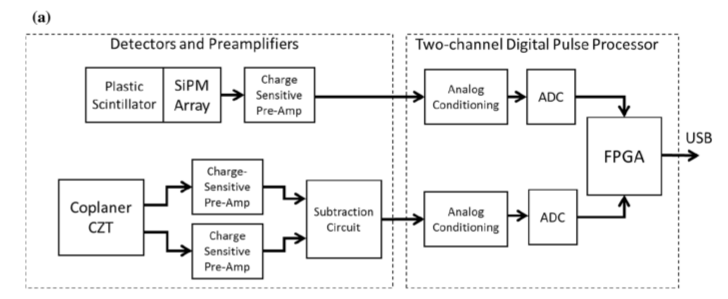
\includegraphics[width=1.0\textwidth]{emsf-08-betagama1.png}
\centering
\caption{Schéma systému pre beta-gama koincidencie.}
\label{em8:fig:betagama1}
\end{figure}

\section{Metóda potláčania Comptonovského rozptylu}
Comptonovské pozadie sa pozoruje, keď sa uskutočňuje Comptonov rozptyl v aktívnom objeme detektora a keď z neho uniknú zodpovedajúce rozptýlené gama lúče. Tieto udalosti predstavujú Comptonovské pozadie. Cieľom anti-comptonovskej koincidencie je snaha potlačiť toto pozadie v spektre. Koincidenčný systém, ktorý je toho schopný pozostáva z dvoch detektorov, kde jeden detektor obklopuje druhy detektor z každej strany. Úlohou detektora, ktorý obklopuje hlavný detektor je zachytávať rozptýlené gama lúče, ktorým sa podarilo uniknúť po rozptyle z hlavného detektora. 

Zvyčajne hlavným detektorom je HPGe detektor, ktorý je obklopený Comptonovským supresorom - bežne sa používajú NaI alebo BGO detektory. NaI detektor poskytuje vynikajúcu časovú odozvu a rozlíšenie ale detektor musí byť dosť veľký. BGO detektor môže byť menší ale má horšie rozlíšenie a časovú odozvu. Avšak energetické rozlíšenie týchto detektorov, ktoré fungujú ako supresory, je v tomto prípade nepodstatné, pretože tieto detektory nepoužívame ako spektrometre. Používame ich totiž len na zistenie, či z hlavného detektora unikol nejaký fotón. Ak áno, tak systém povie hlavnému detektoru aby nespracovával daný signál. Zvyčajnou geometriou supresorového detektora je hrubá stenová trubica, ktorá sa nazýva prstencový detektor. Na jednom konci otvoru je HPGe detektor, druhý koniec je uzavretý tzv. "plug" detektorom. Medzi týmto plug detektorom a HPGe detektorom sa nachádza meraná vzorka. Aby sa dosiahla lepšia redukcia Comptonovskeho pozadia, celý systém je umiestnený vo vnútri pasívneho štítu. Schému anticomptonovského koincidenčného systému je znázornená na obrázku (\ref{em8:fig:anticomton}).

\begin{figure}[!h]
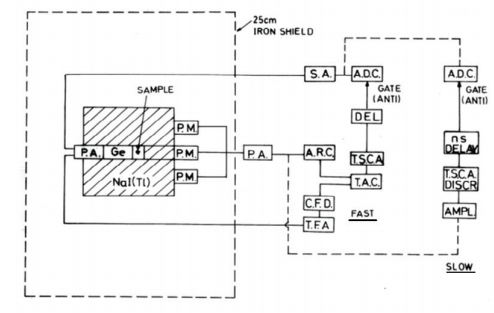
\includegraphics[width=0.8\textwidth]{emsf-08-anticompton.png}
\centering
\caption{Schéma systému pre anticomptonovské koincidencie.}
\label{em8:fig:anticomton}
\end{figure}

\section{Gama-gama koincidenčný detektor - PET}
O tejto metóde sme už písali v sekcii subatómová fyzika a preto nebudeme túto metódu veľmi rozoberať ale zameriame sa len na fyzikálny princíp.

Pozitrónová emisná tomografia (PET) je založená na koincidencii gama-gama. Presnejšie PET systém využíva koincidenčnú detekciu $511\,keV$ fotónov z anihilácie elektrónu s pozitrónom. Keďže spárované gama lúče z anhilácie pozitrónu sú anti-paralelné, detekcia gama lúčov určuje líniu odozvy (line of response - LOR), ktorá vznikla pri anihilácii. Typicky sú PET systémy založené na pevných scintilátoroch (BGO, LSO, ...) a foto detektoroch (PMT, foto-dióda). Na obrázku (\ref{em8:fig:PET}) je znázornená typická geometria PET systému. Skúmaný predmet, ktorý sa skenuje, je obvykle obklopený prstencom, ktorý je zložený z detektorov. Každý detektor zaznamenáva jednotlivé udalosti gama žiarenia a generuje časovaný impulz, ktorý je spojený s každým dopadajúcim fotónom. Tieto impulzy sa potom skombinujú v koincidenčnom obvode, aby sa vybrali spárované gama lúče z rovnakého anihilačného procesu.

\begin{figure}[!h]
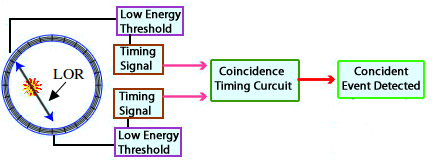
\includegraphics[width=0.8\textwidth]{emsf-08-PET.png}
\centering
\caption{Schéma systému pre PET systém.}
\label{em8:fig:PET}
\end{figure}

\section{Meranie absolútnej aktivity pomocou koincidencii}
Ako ďalšiu aplikáciu koincidenčného obvodu rozoberieme problém merania absolútnej aktivity rádioizotopového zdroja. Ak takýto zdroj emituje dve rozlíšiteľné koincidenčné žiarenia, je možné použiť metódu, pomocou ktorej sa dá spočítať aktivita zdroja bez znalosti absolútnej detekčnej účinnosti detektora. Keďže tieto účinnosti sú často neisté alebo ťažko určiteľné, použitie tejto metódy poskytuje presnejšie výsledky. 

Predpokladajme aktivitu zdroja $A$, ktorý vysiela dve koincidenčné žiarenia, ktoré nie sú vzájomne nijako korelované, čo sa týka uhla emisie. Nastavíme dva detektory tak, že prvý detektor bude zaznamenávať pulzy len od prvého žiarenia, druhý detektor od druhého žiarenia. Výstup týchto detektorov po príslušnom spracovaní pulzov je uvedený do koincidencie s rozhodujúcim časom $\tau$. 

Počet detekcii $r_1$ v prvom detektore môžme napísať ako súčin aktivity $A$ a celkovej efektivity namerania prvého žiarenia $\epsilon_1$. Táto efektivita zahrňuje priestorový uhol, v ktorom sa nachádza detektor, pravdepodobnosť interakcie v detektore a podiel pulzov akceptovaných následným obvodom. Podobný vzťah platí aj pre druhé žiarenie a preto môžme písať
$$ r_1 = A \epsilon_1 $$ 
$$ r_2 = A \epsilon_2 $$
Mieru pravej koincidencie $r_t$ môžme predpovedať vďaka znalosti, že musí dôjsť ku dvom udalostiam: žiarenie 1 sa detekuje v prvom detektore, žiarenie 2 v druhom. Nezávislé pravdepodobnosti (nezávisle preto lebo tieto žiarenia nie sú uhlovo korelované) jednotlivých detekcii sú $\epsilon_1$ a $\epsilon_2$, tak potom pravdepodobnosť, že dôjde k detekcii prvej a zároveň aj druhej udalosti bude $\epsilon_1 \epsilon_2$. Miera pravej koincidencie je tak súčinom tejto kombinovanej pravdepodobnosti a aktivity zdroja $A$,
$$ r_t = A \epsilon_1 \epsilon_2.$$
Meraná miera koincidencie $r_{12}$ je súčtom pravej miery koincidencie $r_t$ a náhodnej miery koincidencie $r_{ch}$
$$ r_{12} = r_t + r_{ch}.$$
Riešením týchto rovníc a elimináciou $\epsilon_1$ a $\epsilon_2$, môžme pre aktivitu písať 
$$ A = \frac{r_1 r_2}{r_t}.$$
Tento vzťah udáva aktivitu zdroja, ktorá je vyjadrená cez početnosti, ktoré vieme merať.

V mnohých prípadoch bývajú dva koincidenčné žiarenia: beta a gama, ($\beta-\gamma$), koincidencia. Tieto žiarenia sú emitované pri rozpade daného izotopu. Ak je jedno žiarenie detekované cez celý priestorový uhol, potom je možné požiadavku uhlovej nezávislosti oboch meraných žiarení vynechať. Bežná sa dá táto metóda realizovať použitím $4\pi$ proporcionálneho počítača ako beta detektor v spojení s detektorom gama žiarenia, ktorý pokrýva menší uhol. Touto metódou je možné dosiahnuť presnosť blížiacu sa jednému percentu.

\section{Sumačný koincidenčný mód}
Väčšina Comptonovho pozadia pochádza z jediného Comptonovho rozptylu, po ktorom nasleduje únik rozptýleného gama žiarenia z detektora, zatiaľ čo plné energetické udalosti pri typických energiách gama-žiarenia sú primárne zložené z niekoľkých rozptýlených sekvencií, po ktorých nasleduje fotoelektrická absorpcia (čiže dochádza k viacnásobnému rozptylu ale žiaden fotón neunikne z detektora, celá energia sa zaznamenáva). Z toho dôvodu môže byť pomer medzi plne energetickým pikom a Comtonovským pozadím zvýšený požiadavkou, aby zaznamenaná udalosť zodpovedala viacerým interakciám (častica sa viackrát rozptýli) vo vnútri detektora a až po viacnásobnom rozptyle dôjde k zaznamenaniu udalosti detektorom. V germániových detektoroch sa táto voľba zvyčajne uskutočňuje rozdelením detektora na niekoľko segmentov (alebo poskytnutím niekoľkých priľahlých nezávislých detektorov) a hľadaním koincidenčných impulzov z dvoch alebo viacerých nezávislých segmentov. Keď sa detekuje koincidencia, výstup zo všetkých segmentov detektora sa spočíta a zaznamená. Výsledné spektrum sa skladá iba z maximálneho energetického vrcholu, ležiaceho nad slabým pozadím, ktoré je výrazne potlačené a nemá žiadne náhlé Comtonovské hrany, viď obrázok (\ref{em8:fig:sumacia}).

\begin{figure}[!h]
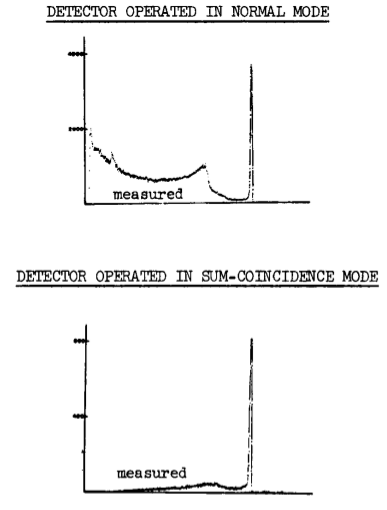
\includegraphics[width=0.6\textwidth]{emsf-08-sumacia.png}
\centering
\caption{Príklad spektra pred a po sumačnom koincidenčnom móde.}
\label{em8:fig:sumacia}
\end{figure}

\section{Párový koincidenčný spektrometer}
Iným prístupom k zjednodušeniu zaznamenaného spektra germániových detektorov je snaha vybrať len piky dvojitého úniku. Ak je energia gama žiarenia dostatočne vysoká, významná časť všetkých interakcií bude zodpovedať výrobe elektrón-pozitrón párov, pri ktorej oba fotóny produkované pozitrónovou anihiláciou uniknú z primárneho detektora. Pretože tieto anihilačné fotóny sú vždy vyemitované v opačnom smere, dva ďalšie detektory umiestnené na protiľahlých stranách primárneho detektora ich môžu zachytiť s rozumnou účinnosťou. Ak sa požaduje koincidencia medzi všetkými troma detektormi, výber dvojitých únikových udalostí bude veľmi špecifický a väčšina kontinua (rovnako ako maximálny energetický vrchol) bude potlačená. Takéto systémy pozostávajú z centrálneho germániového detektora a dvoch okolitých NaI(Tl) alebo BGO scintilátorov. Poloha tohto double piku na energetickej osy je daná nasledovne
$$ E_{doublepeak} = hf - 1022\,keV.$$
kde $hf$ je počiatočná energia vchádzajúceho gama žiarenia.

Na obrázku môžme vidieť príklad spektra pre párový spektrometer. Hoci väčšina zaznamenaných udalostí zodpovedá izolovanému dvojitému únikovému piku, malé pozadie stále pretrváva v dôsledku niekoľkých neideálnosti. 

\begin{figure}[!h]
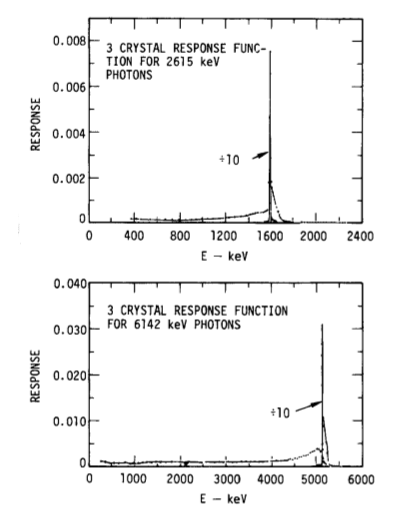
\includegraphics[width=0.6\textwidth]{emsf-08-pair.png}
\centering
\caption{Príklad spektra pre párovú koincidenciu.}
\label{em8:fig:pair}
\end{figure}

Impulzy napravo od piku sa dajú zaznamenať z udalostí, pri ktorých sa anihilačný fotón podrobí malému rozptylu pred opustením centrálneho detektora (tým sa zaznamenaná energia zvýši o malinky kúsoček), ale stále bude tento fotón spadat do akceptovateľného impulzového výškového okienka vonkajších detektorov a preto bude zaznamenaná koincidencia. Udalosti na ľavej strane piku môžu byť generované interakciami gama-žiarenia, ktoré sa vyskytujú v blízkosti hranice centrálneho detektora a pre ktoré uniká buď pozitrón alebo elektrónov bez uloženia celej svojej energie do detektora.
















\end{document}